\documentclass[12pt,preprint, authoryear]{elsarticle}

\usepackage{lmodern}
%%%% My spacing
\usepackage{setspace}
\setstretch{1.5}
\DeclareMathSizes{12}{14}{10}{10}

% Wrap around which gives all figures included the [H] command, or places it "here". This can be tedious to code in Rmarkdown.
\usepackage{float}
\let\origfigure\figure
\let\endorigfigure\endfigure
\renewenvironment{figure}[1][2] {
    \expandafter\origfigure\expandafter[H]
} {
    \endorigfigure
}

\let\origtable\table
\let\endorigtable\endtable
\renewenvironment{table}[1][2] {
    \expandafter\origtable\expandafter[H]
} {
    \endorigtable
}


\usepackage{ifxetex,ifluatex}
\usepackage{fixltx2e} % provides \textsubscript
\ifnum 0\ifxetex 1\fi\ifluatex 1\fi=0 % if pdftex
  \usepackage[T1]{fontenc}
  \usepackage[utf8]{inputenc}
\else % if luatex or xelatex
  \ifxetex
    \usepackage{mathspec}
    \usepackage{xltxtra,xunicode}
  \else
    \usepackage{fontspec}
  \fi
  \defaultfontfeatures{Mapping=tex-text,Scale=MatchLowercase}
  \newcommand{\euro}{€}
\fi

\usepackage{amssymb, amsmath, amsthm, amsfonts}

\def\bibsection{\section*{References}} %%% Make "References" appear before bibliography


\usepackage[round]{natbib}

\usepackage{longtable}
\usepackage[margin=2.3cm,bottom=2cm,top=2.5cm, includefoot]{geometry}
\usepackage{fancyhdr}
\usepackage[bottom, hang, flushmargin]{footmisc}
\usepackage{graphicx}
\numberwithin{equation}{section}
\numberwithin{figure}{section}
\numberwithin{table}{section}
\setlength{\parindent}{0cm}
\setlength{\parskip}{1.3ex plus 0.5ex minus 0.3ex}
\usepackage{textcomp}
\renewcommand{\headrulewidth}{0.2pt}
\renewcommand{\footrulewidth}{0.3pt}

\usepackage{array}
\newcolumntype{x}[1]{>{\centering\arraybackslash\hspace{0pt}}p{#1}}

%%%%  Remove the "preprint submitted to" part. Don't worry about this either, it just looks better without it:
\makeatletter
\def\ps@pprintTitle{%
  \let\@oddhead\@empty
  \let\@evenhead\@empty
  \let\@oddfoot\@empty
  \let\@evenfoot\@oddfoot
}
\makeatother

 \def\tightlist{} % This allows for subbullets!

\usepackage{hyperref}
\hypersetup{breaklinks=true,
            bookmarks=true,
            colorlinks=true,
            citecolor=blue,
            urlcolor=blue,
            linkcolor=blue,
            pdfborder={0 0 0}}


% The following packages allow huxtable to work:
\usepackage{siunitx}
\usepackage{multirow}
\usepackage{hhline}
\usepackage{calc}
\usepackage{tabularx}
\usepackage{booktabs}
\usepackage{caption}


\newenvironment{columns}[1][]{}{}

\newenvironment{column}[1]{\begin{minipage}{#1}\ignorespaces}{%
\end{minipage}
\ifhmode\unskip\fi
\aftergroup\useignorespacesandallpars}

\def\useignorespacesandallpars#1\ignorespaces\fi{%
#1\fi\ignorespacesandallpars}

\makeatletter
\def\ignorespacesandallpars{%
  \@ifnextchar\par
    {\expandafter\ignorespacesandallpars\@gobble}%
    {}%
}
\makeatother

\newlength{\cslhangindent}
\setlength{\cslhangindent}{1.5em}
\newenvironment{CSLReferences}%
  {\setlength{\parindent}{0pt}%
  \everypar{\setlength{\hangindent}{\cslhangindent}}\ignorespaces}%
  {\par}


\urlstyle{same}  % don't use monospace font for urls
\setlength{\parindent}{0pt}
\setlength{\parskip}{6pt plus 2pt minus 1pt}
\setlength{\emergencystretch}{3em}  % prevent overfull lines
\setcounter{secnumdepth}{5}

%%% Use protect on footnotes to avoid problems with footnotes in titles
\let\rmarkdownfootnote\footnote%
\def\footnote{\protect\rmarkdownfootnote}
\IfFileExists{upquote.sty}{\usepackage{upquote}}{}

%%% Include extra packages specified by user

%%% Hard setting column skips for reports - this ensures greater consistency and control over the length settings in the document.
%% page layout
%% paragraphs
\setlength{\baselineskip}{12pt plus 0pt minus 0pt}
\setlength{\parskip}{12pt plus 0pt minus 0pt}
\setlength{\parindent}{0pt plus 0pt minus 0pt}
%% floats
\setlength{\floatsep}{12pt plus 0 pt minus 0pt}
\setlength{\textfloatsep}{20pt plus 0pt minus 0pt}
\setlength{\intextsep}{14pt plus 0pt minus 0pt}
\setlength{\dbltextfloatsep}{20pt plus 0pt minus 0pt}
\setlength{\dblfloatsep}{14pt plus 0pt minus 0pt}
%% maths
\setlength{\abovedisplayskip}{12pt plus 0pt minus 0pt}
\setlength{\belowdisplayskip}{12pt plus 0pt minus 0pt}
%% lists
\setlength{\topsep}{10pt plus 0pt minus 0pt}
\setlength{\partopsep}{3pt plus 0pt minus 0pt}
\setlength{\itemsep}{5pt plus 0pt minus 0pt}
\setlength{\labelsep}{8mm plus 0mm minus 0mm}
\setlength{\parsep}{\the\parskip}
\setlength{\listparindent}{\the\parindent}
%% verbatim
\setlength{\fboxsep}{5pt plus 0pt minus 0pt}



\begin{document}



\begin{frontmatter}  %

\title{Question 3}

% Set to FALSE if wanting to remove title (for submission)




\author[Add1]{Sahil Bhugwan}
\ead{21075492@sun.ac.za}





\address[Add1]{Github- \url{https://github.com/SBhugwan}}


\begin{abstract}
\small{
The two longest Bands of all time Coldplay and Metallica. Comparing
these two bands on longevity and musical progression
}
\end{abstract}

\vspace{1cm}


\begin{keyword}
\footnotesize{
music\textbackslash{} \\
\vspace{0.3cm}
}
\end{keyword}



\vspace{0.5cm}

\end{frontmatter}



%________________________
% Header and Footers
%%%%%%%%%%%%%%%%%%%%%%%%%%%%%%%%%
\pagestyle{fancy}
\chead{}
\rhead{}
\lfoot{}
\rfoot{\footnotesize Page \thepage}
\lhead{}
%\rfoot{\footnotesize Page \thepage } % "e.g. Page 2"
\cfoot{}

%\setlength\headheight{30pt}
%%%%%%%%%%%%%%%%%%%%%%%%%%%%%%%%%
%________________________

\headsep 35pt % So that header does not go over title




\hypertarget{introduction}{%
\section{\texorpdfstring{Introduction
\label{Introduction}}{Introduction }}\label{introduction}}

In this report i will be looking at the two most famous bands of all
time that being coldplay and Metallica. i will be looking at a variety
of analysis to come the two bands. First i will be looking at Coldplay
then Metallica.

\hypertarget{coldplay}{%
\section*{Coldplay}\label{coldplay}}
\addcontentsline{toc}{section}{Coldplay}

The first thing is i will be looking at when coldplay become popular.

\begin{figure}[H]

{\centering \includegraphics{Q3_files/figure-latex/Figure1-1} 

}

\caption{Popularity of Songs \label{Figure1}}\label{fig:Figure1}
\end{figure}

It is clear from this that from the time coldplay came into the scene
they where popular already, however during the early 2010s that is when
there popularity became prominant this could be because of certain songs
they released.

\begin{figure}[H]

{\centering \includegraphics{Q3_files/figure-latex/Figure2-1} 

}

\caption{Songs over time  \label{Figure2}}\label{fig:Figure2}
\end{figure}

\begin{verbatim}
## $cold_pop
## # A tibble: 10 x 16
##    name        durat~1 release_~2 album~3 expli~4 popul~5 acous~6 dance~7 energy
##    <chr>         <dbl> <date>     <chr>   <lgl>     <dbl>   <dbl>   <dbl>  <dbl>
##  1 A Head Ful~    294. 2018-12-07 Love i~ FALSE        14 0.0948    0.307  0.92 
##  2 A Head Ful~    224. 2015-12-04 A Head~ FALSE        70 0.0021    0.449  0.92 
##  3 Hymn for t~    258. 2015-12-04 A Head~ FALSE        86 0.211     0.491  0.693
##  4 Adventure ~    264. 2015-12-04 A Head~ FALSE        80 0.00205   0.638  0.924
##  5 A Head Ful~    224. 2015-12-04 A Head~ FALSE        18 0.0021    0.449  0.92 
##  6 Hymn for t~    258. 2015-12-04 A Head~ FALSE        26 0.211     0.491  0.693
##  7 Adventure ~    264. 2015-12-04 A Head~ FALSE        23 0.00205   0.638  0.924
##  8 Viva La Vi~    242. 2008-11-24 Viva L~ FALSE        34 0.0954    0.486  0.617
##  9 Viva La Vi~    242. 2008-06-19 Viva L~ FALSE        75 0.0954    0.486  0.617
## 10 Yellow         267. 2000-07-10 Parach~ FALSE        91 0.00239   0.429  0.661
## # ... with 7 more variables: instrumentalness <dbl>, liveness <dbl>,
## #   loudness <dbl>, speechiness <dbl>, tempo <dbl>, valence <dbl>,
## #   album_release <date>, and abbreviated variable names 1: duration,
## #   2: release_date, 3: album_name, 4: explicit, 5: popularity,
## #   6: acousticness, 7: danceability
## 
## $order
##  [1] "Parachutes"                               
##  [2] "A Rush of Blood to the Head"              
##  [3] "A Head Full of Dreams"                    
##  [4] "Ghost Stories"                            
##  [5] "Music Of The Spheres"                     
##  [6] "X&Y"                                      
##  [7] "Live in Buenos Aires"                     
##  [8] "Mylo Xyloto"                              
##  [9] "Live 2012"                                
## [10] "Ghost Stories Live 2014"                  
## [11] "Viva La Vida or Death and All His Friends"
## [12] "Live 2003"                                
## [13] "LeftRightLeftRightLeft (Live)"            
## [14] "Viva La Vida (Prospekts March Edition)"   
## [15] "Everyday Life"                            
## [16] "A Head Full of Dreams Tour Edition"       
## [17] "Love in Tokyo"
\end{verbatim}

It is clear from \ref{Figure2} that they really hit there stride in the
late 2010s as twice in in one album they had 3 top songs

Next looking at there correlation matrix to assess certain apsects of
there music

\begin{figure}[H]

{\centering 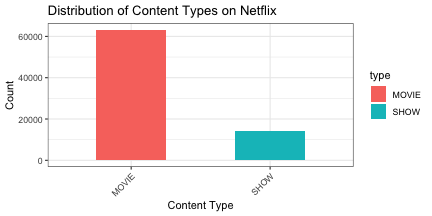
\includegraphics{Q3_files/figure-latex/Figure3-1} 

}

\caption{Correlation matrix  \label{Figure1}}\label{fig:Figure3}
\end{figure}

\hypertarget{mettallica}{%
\section{Mettallica}\label{mettallica}}

Next i will be looking at Mettallica. they also have been a very long
perfroming band. Though it must be noted that they do perform different
music to that of coldplay.

I once again will be looking at the scatter plot to see there popularity

\begin{figure}[H]

{\centering \includegraphics{Q3_files/figure-latex/Figure4-1} 

}

\caption{Popularity of Songs \label{Figure1}}\label{fig:Figure4}
\end{figure}

It is clear that mettalica where he most popular during the late 1980s.
However they appeared to be less popular between 2000 and 2010 however
they started gaining moment in early 2020s.

Next i will also be looking at the most popular songs

\begin{figure}[H]

{\centering \includegraphics{Q3_files/figure-latex/Figure5-1} 

}

\caption{Songs over time  \label{Figure5}}\label{fig:Figure5}
\end{figure}

\begin{verbatim}
## $cold_pop
## # A tibble: 10 x 15
##    name        album~1 durat~2 popul~3 release_~4 dance~5 energy loudn~6 speec~7
##    <chr>       <chr>     <dbl>   <dbl> <date>       <dbl>  <dbl>   <dbl>   <dbl>
##  1 Turn The P~ Garage~  366400      62 1998-11-24   0.422  0.818   -3.94  0.0319
##  2 Whiskey In~ Garage~  304893      67 1998-11-24   0.511  0.972   -3.75  0.0413
##  3 Turn The P~ Garage~  366467      66 1998-01-01   0.426  0.813   -3.96  0.0318
##  4 Whiskey In~ Garage~  304693      76 1998-01-01   0.511  0.97    -3.72  0.0414
##  5 One (Remas~ ...And~  446146      51 1988-09-07   0.438  0.687   -9.15  0.0619
##  6 One (Remas~ ...And~  446146      72 1988-09-07   0.438  0.687   -9.15  0.0619
##  7 One         And Ju~  446146      50 1988-08-25   0.439  0.691   -9.16  0.0608
##  8 One         ...And~  447440      75 1988-08-25   0.437  0.695   -9.45  0.0617
##  9 For Whom T~ Ride T~  309973      73 1984-07-27   0.512  0.86    -6.14  0.0703
## 10 For Whom T~ Ride T~  309973      54 1984-07-27   0.512  0.86    -6.14  0.0703
## # ... with 6 more variables: acousticness <dbl>, instrumentalness <dbl>,
## #   liveness <dbl>, valence <dbl>, tempo <dbl>, album_release <date>, and
## #   abbreviated variable names 1: album_name, 2: duration_ms, 3: popularity,
## #   4: release_date, 5: danceability, 6: loudness, 7: speechiness
## 
## $order
##  [1] "72 Seasons"                                                 
##  [2] "Metallica"                                                  
##  [3] "Metallica (Remastered)"                                     
##  [4] "Master Of Puppets (Remastered)"                             
##  [5] "...And Justice For All"                                     
##  [6] "Kill Em All (Remastered)"                                   
##  [7] "...And Justice for All (Remastered)"                        
##  [8] "Ride The Lightning (Remastered)"                            
##  [9] "Death Magnetic"                                             
## [10] "Garage Inc."                                                
## [11] "HardwiredTo Self-Destruct"                                  
## [12] "Load"                                                       
## [13] "And Justice for All (Remastered)"                           
## [14] "Metallica (Remastered 2021)"                                
## [15] "Reload"                                                     
## [16] "Garage, Inc."                                               
## [17] "HardwiredTo Self-Destruct (Deluxe)"                         
## [18] "Metallica Through The Never (Music From The Motion Picture)"
## [19] "St. Anger"                                                  
## [20] "S&M2"                                                       
## [21] "S&M"                                                        
## [22] "Live Sh*t: Binge & Purge (Live In Mexico City)"             
## [23] "Helping HandsLive & Acoustic At The Masonic"                
## [24] "Live S**t: Binge & Purge"                                   
## [25] "Ride The Lightning (Deluxe Remaster)"                       
## [26] "Some Kind Of Monster"                                       
## [27] "Ride The Lightning (Deluxe / Remastered)"                   
## [28] "Helping Hands...Live & Acoustic at The Masonic"             
## [29] "Live In Brazil (1993 \x93 2017)"                            
## [30] "Kill Em All (Deluxe / Remastered)"                          
## [31] "Metallica (Remastered Deluxe Box Set)"                      
## [32] "Lulu"                                                       
## [33] "Kill Em All (Deluxe Remaster)"                              
## [34] "Master of Puppets (Remastered Deluxe Box Set)"              
## [35] "And Justice for All (Remastered Deluxe Box Set)"            
## [36] "...And Justice for All (Remastered Deluxe Box Set)"         
## [37] "Some Kind Of Monster (Live)"                                
## [38] "Live In Chile (1993 \x93 2017)"                             
## [39] "Master Of Puppets (Deluxe Box Set / Remastered)"            
## [40] "Live In Argentina (1993 \x93 2017)"                         
## [41] "Six Feet Down Under Part 2"                                 
## [42] "Six Feet Down Under"
\end{verbatim}

It can be seen they they clearly peaked in the late 1990s

lastly i will be looking at the correlation matrix for metallica

\begin{figure}[H]

{\centering \includegraphics{Q3_files/figure-latex/Figure6-1} 

}

\caption{Correlation matrix  \label{Figure6}}\label{fig:Figure6}
\end{figure}

Now if we had to look at the song duration between coldplay and
mettallica

\begin{figure}[H]

{\centering \includegraphics{Q3_files/figure-latex/Figure7-1} 

}

\caption{Song Duration   \label{Figure7}}\label{fig:Figure7}
\end{figure}

\hypertarget{extra}{%
\section{Extra}\label{extra}}

Next I want to analyse the different genres i how much energy the
produce

\begin{figure}[H]

{\centering \includegraphics{Q3_files/figure-latex/Figure8-1} 

}

\caption{Engergy per Genre  \label{Figure8}}\label{fig:Figure8}
\end{figure}

It is clear from this that metal and punk will give you the most energy

\hypertarget{conclusion}{%
\section{Conclusion}\label{conclusion}}

Coldplay and Metallica are two great bands but obviously they have
different target audiences. These will depend on an individuals tastes
which will affect there popularity.

\bibliography{Tex/ref}





\end{document}
